\documentclass[border=3pt,tikz]{standalone}
% Shared look for every TikZ figure in these notes.
% Included by each standalone figure file; also keeps the figures consistent
% with the colours used in the PDF and on the website.

\usepackage{tikz}
\usepackage{pgfplots}
\pgfplotsset{compat=1.18}
\usetikzlibrary{arrows.meta, decorations.markings, decorations.pathmorphing,
                patterns, calc, positioning}
\usepackage{amsmath}

% Series colours are the three validated categorical slots also used by the
% interactive widgets, so a path drawn in the printed notes and the same path on
% the website are the same colour. They clear the colour-vision-deficiency and
% contrast checks as a set; every path is direct-labelled as well, so colour is
% never the only thing carrying identity.
\definecolor{duPurple}{HTML}{68246D}
\definecolor{duBlue}{HTML}{2A78D6}
\definecolor{duRed}{HTML}{EB6834}
\definecolor{duGreen}{HTML}{1BAF7A}
\definecolor{duGrey}{HTML}{6B6B6B}

\tikzset{
  axisline/.style   = {-{Stealth[length=3mm]}, line width=0.7pt, black},
  path1/.style      = {duBlue,   line width=1.1pt},
  path2/.style      = {duRed,    line width=1.1pt},
  path3/.style      = {duGreen,  line width=1.1pt},
  statedot/.style   = {circle, fill=black, inner sep=1.4pt},
  arrowhead/.style  = {decoration={markings,
                        mark=at position #1 with {\arrow{Stealth[length=2.6mm]}}},
                       postaction={decorate}},
  lbl/.style        = {font=\small},
  slbl/.style       = {font=\footnotesize, duGrey},
  workfill/.style   = {duPurple, opacity=0.16},
}

\begin{document}
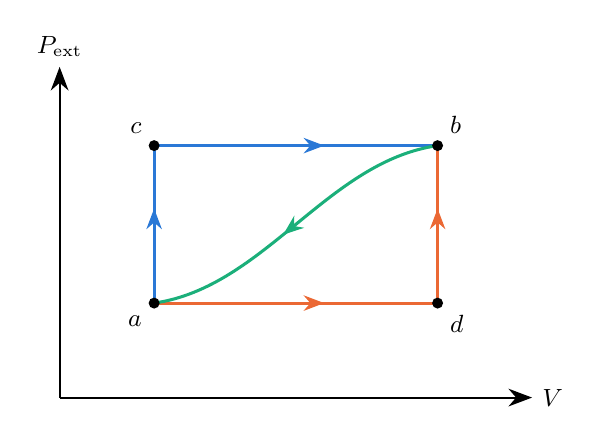
\begin{tikzpicture}[scale=1]
  \draw[axisline] (0,0) -- (6.0,0) node[right, lbl] {$V$};
  \draw[axisline] (0,0) -- (0,4.2) node[above, lbl] {$P_\text{ext}$};

  \coordinate (a) at (1.2,1.2);
  \coordinate (b) at (4.8,3.2);
  \coordinate (c) at (1.2,3.2);
  \coordinate (d) at (4.8,1.2);

  % path a-c-b (via c, i.e. up then across)
  \draw[path1, arrowhead=0.6] (a) -- (c);
  \draw[path1, arrowhead=0.6] (c) -- (b);
  % path a-d-b (via d, i.e. across then up)
  \draw[path2, arrowhead=0.6] (a) -- (d);
  \draw[path2, arrowhead=0.6] (d) -- (b);
  % the curved return path b -> a
  \draw[path3, arrowhead=0.55] (b) .. controls (3.4,3.0) and (2.6,1.4) .. (a);

  \node[statedot] at (a) {}; \node[lbl, below left  = 1pt and 1pt] at (a) {$a$};
  \node[statedot] at (b) {}; \node[lbl, above right = 1pt and 1pt] at (b) {$b$};
  \node[statedot] at (c) {}; \node[lbl, above left  = 1pt and 1pt] at (c) {$c$};
  \node[statedot] at (d) {}; \node[lbl, below right = 1pt and 1pt] at (d) {$d$};
\end{tikzpicture}
\end{document}
